%* 
%* ------------------------------------------------------------------
%* AN02_TheLayout.tex - Application Note 02: The Layout
%* Created by Robert Heller on Thu Sep 20 08:40:38 2012
%* ------------------------------------------------------------------
%* Modification History: $Log$
%* Modification History: Revision 1.1  2002/07/28 14:03:50  heller
%* Modification History: Add it copyright notice headers
%* Modification History:
%* ------------------------------------------------------------------
%* Contents:
%* ------------------------------------------------------------------
%*  
%*     Model RR System, Version 2
%*     Copyright (C) 1994,1995,2002-2012  Robert Heller D/B/A Deepwoods Software
%* 			51 Locke Hill Road
%* 			Wendell, MA 01379-9728
%* 
%*     This program is free software; you can redistribute it and/or modify
%*     it under the terms of the GNU General Public License as published by
%*     the Free Software Foundation; either version 2 of the License, or
%*     (at your option) any later version.
%* 
%*     This program is distributed in the hope that it will be useful,
%*     but WITHOUT ANY WARRANTY; without even the implied warranty of
%*     MERCHANTABILITY or FITNESS FOR A PARTICULAR PURPOSE.  See the
%*     GNU General Public License for more details.
%* 
%*     You should have received a copy of the GNU General Public License
%*     along with this program; if not, write to the Free Software
%*     Foundation, Inc., 675 Mass Ave, Cambridge, MA 02139, USA.
%* 
%*  
%* 

\chapter{The Layout}
\label{chapt:TheLayout}
\typeout{$Id$}

\begin{figure}[hbpt]
\begin{centering}
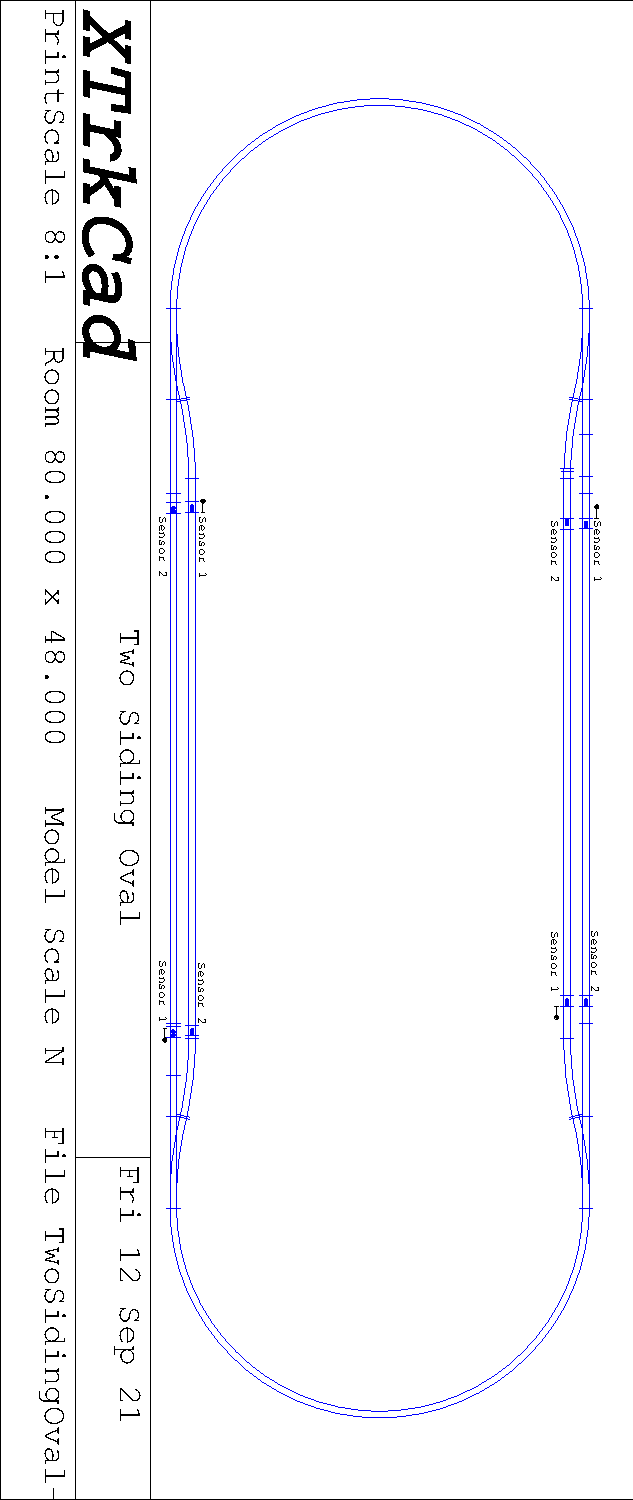
\includegraphics[angle=90,width=5in]{TwoSidingOval-N.pdf}
\caption{Two Siding Oval N}
\label{fig:TheLayout:TwoSidingOval-N}
\end{centering}
\end{figure}
The complete layout is shown in
Figure~\ref{fig:TheLayout:TwoSidingOval-N}. This is a basic oval with a
pair of passing sidings, one on each straight section. The turnouts at
the ends of the passing sidings will be controled by the computer to
allow continious running of two trains going in \textit{opposite}
directions.  If necessary, a train will be held at the end of its
siding until the other train clears the single track segment. The
computer will use Azatrax MRD2-U IR sensors to sense when the single
track segments are occupied and will use Azatrax SR4-U modules to
control the  direction of travel on the single track segments as well
as energizing the twin-coil switch machines to throw the turnouts as
needed. The trains will be plain DC powered and the rails will have gaps
to isolate the various power sections.  The single track segments will
be powered from computer controlled reversing relays since these segments
will be operating in alternating directions.  The sidings will be fixed
polarity wired.

\begin{figure}[hbpt]
\begin{centering}
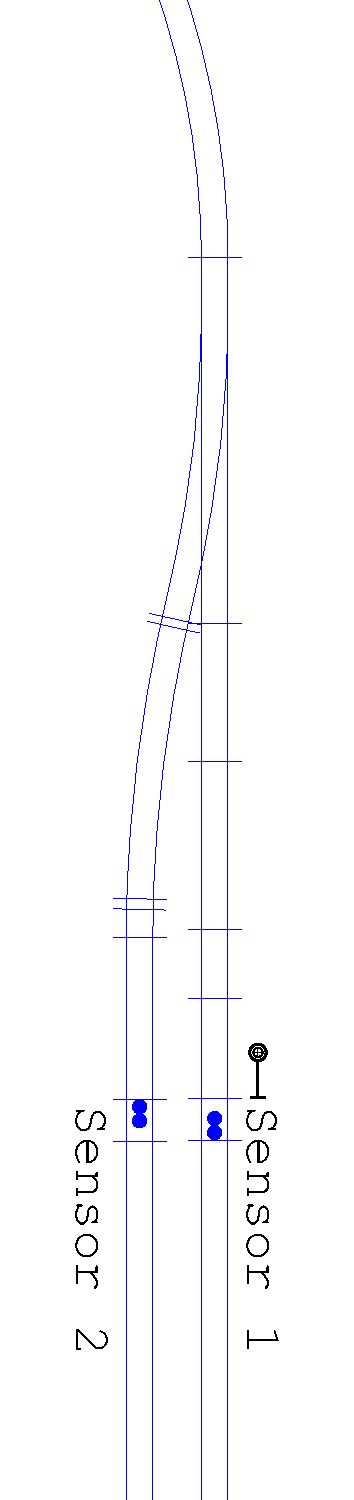
\includegraphics[angle=90,width=5in]{TwoSidingOval-N-NW-Switch-sig-sensor.pdf}
\caption{Two Siding Oval N, North West Switch with Signal and Sensor locations.}
\label{fig:TheLayout:TwoSidingOval-N-NW-Switch-sig-sensor}
\end{centering}
\end{figure}
\begin{figure}[hbpt]
\begin{centering}
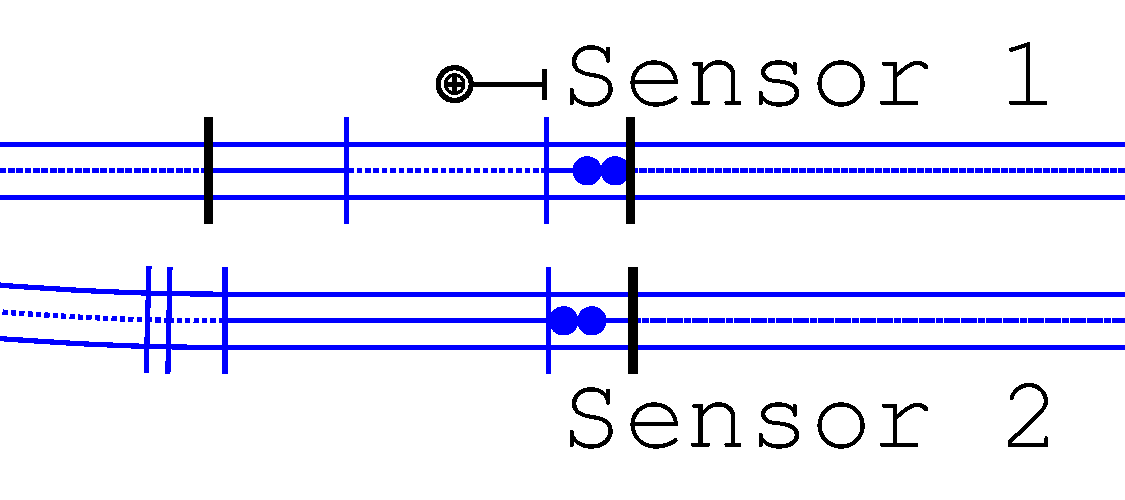
\includegraphics[width=5in]{TwoSidingOval-N-NW-sig-sensor-detail.pdf}
\caption{Two Siding Oval N, North West Signal and Sensor detail, with gaps.}
\label{fig:TheLayout:TwoSidingOval-N-NW-sig-sensor-detail}
\end{centering}
\end{figure}
\begin{figure}[hbpt]
\begin{centering}
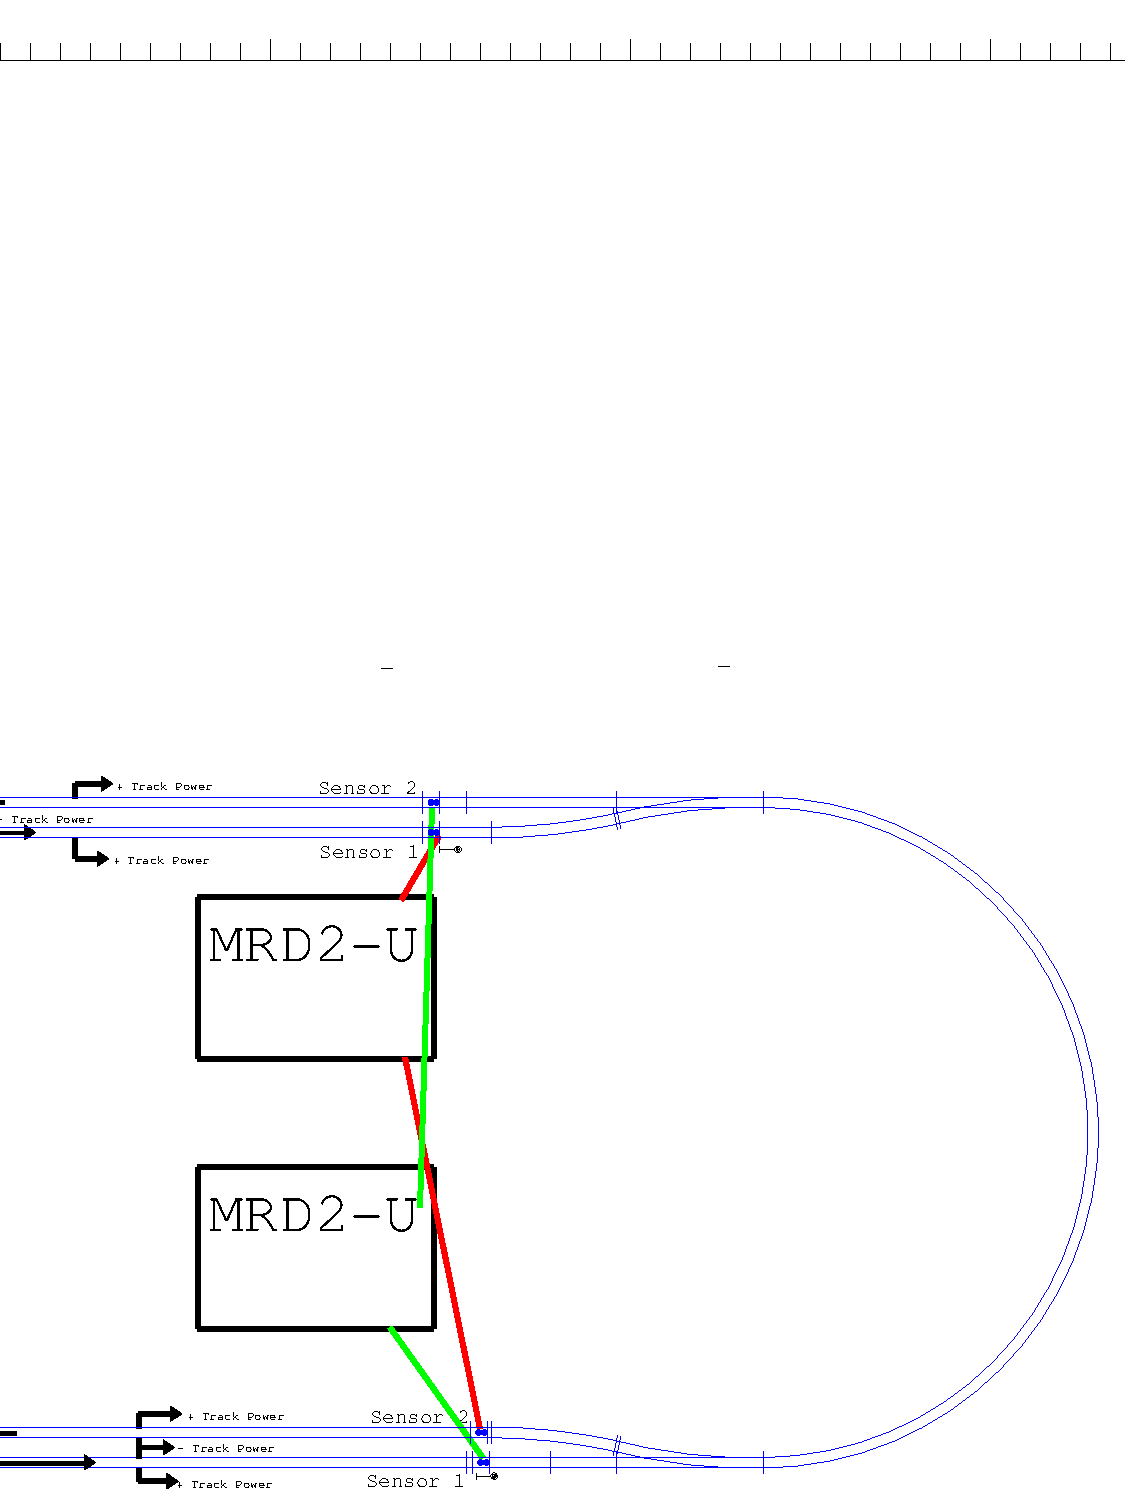
\includegraphics[width=5in]{TwoSidingOval-N-East-MRD2.pdf}
\caption{Two Siding Oval N, East Sensor connections for MRD2-U modules.}
\label{fig:TheLayout:TwoSidingOval-N-East-MRD2}
\end{centering}
\end{figure}
Figures~\ref{fig:TheLayout:TwoSidingOval-N-NW-Switch-sig-sensor} and
\ref{fig:TheLayout:TwoSidingOval-N-NW-sig-sensor-detail} show the
detail of the North West Switch with the signal and sensor locations.
This is typical for each corner. The inner siding is clockwise running
and the outer siding is counter clockwise running\footnote{This happens
to correspond to ``right hand'' running.}.  There are eight sensor
locations, two for each MRD2-U module. 
Figure~\ref{fig:TheLayout:TwoSidingOval-N-East-MRD2} shows how the
East end sensors are connected.  The West end follows a similar
pattern. Sensor one for each MRD2-U is the sensor at the entrance end
of each logical route through the single track main lines, located at
the signal (just before the turnout) and sensor two for that MRD2-U is
the sensor at the exit of that logical route through the single track
main line (just after the turnout). The end curves handle bi-direction
traffic and each MRD2-U device detects trains going in a specific
direction.  If the software determines that the route is occupied by a
train going in one direction, it will hold the train going in the other
direction until the first train clears the exit sensor. If the entrance
sensor detects a train (which will be stopped at the sensor/signal), the
software will change the turnout alignment and flip the direction of
travel and will hold opposing traffic. 

